    \section{正交性orthogonality}
    \subsection{4个子空间的正交性}
    当b在列空间之外时(当我们想要求解Ax = b而不能这样做时)那么$A^T$的这个零空间就会自成一体。 它包含“最小二乘”解决方案中的误差$e = b-Ax$。最小二乘法是本章线性代数的关键应用。
    \\
    同一个向量空间的两个子空间V,W有 \textbf{V与W是正交的}:$\boldsymbol{v}^{\mathrm{T}} \boldsymbol{w}=0$ for all $\boldsymbol{v}$ in $\boldsymbol{V}$ and all $\boldsymbol{w}$ in $\boldsymbol{W}$
    \\
    注意:一定是子空间中的每个向量!比如三维空间中的两个垂直的平面,因为它们的交线不能垂直于自己,所以这两个平面不是正交的!
    \\
    若有一个向量能同时处于两个正交子空间中,则这个向量必定是\textbf{零向量},零向量垂直于自己。\\
    当$\operatorname{dim} V+\operatorname{dim} W>\operatorname{dim}(\text { whole space })$,$V$和$W$\textbf{不可能正交}!
    \\
    Every vector $x$ in the nullspace is perpendicular to every row of $A,$ because $A x=0$ .\\
    The nullspace $N(A)$ and the row space $C\left(A^{T}\right)$ are orthogonal subspaces of $\mathbf{R}^{n}$ .$C(A^T) \perp N\left(A \right)$
    \\
    2 proof:
    \begin{itemize}
        \item $A \boldsymbol{x}=\left[\begin{array}{c}{\operatorname{row} 1} \\ {\vdots} \\ {\operatorname{row} m}\end{array}\right][\boldsymbol{x}]=\left[\begin{array}{c}{0} \\ {\vdots} \\ {0}\end{array}\right]$,Every row has a zero dot product with $\bm{x}$. Then $\bm{x}$ is also perpendicular
to every combination of the rows.
        \item 行空间中的向量是行的线性组合$A^T\bm{y}$,\quad $\bm{x}$则是零空间的向量,则有$\boldsymbol{x}^{\mathrm{T}}\left(A^{\mathrm{T}} \boldsymbol{y}\right)=(A \boldsymbol{x})^{\mathrm{T}} \boldsymbol{y}=\mathbf{0}^{\mathrm{T}} \boldsymbol{y}=0$.
    \end{itemize}
    Every vector $y$ in the nullspace of $A^{\mathrm{T}}$ is perpendicular to every column of $A$\\
    The left nullspace $N\left(A^{\mathrm{T}}\right)$ and the column space $C(A)$ are orthogonal in $\mathbf{R}^{m}$, $C(A) \perp N\left(A^{\mathrm{T}}\right)$.
    \\
    \subsection{正交补orthogonal complements}
    定义:一个子空间V的\textbf{正交补包含了每一条垂直于V的向量},这个正交空间记为:$V^\perp$.\\
    例子:零空间是行空间的正交补,每一条垂直于行空间的向量都满足$A\bm{x}=\bm{0}$,且均处于零空间中。它们满足$r+(n-r)=n$。列空间和左零空间同理!
    \\
    \begin{itemize}
        \item 零空间$\mathbf{N}(A)$是行空间$\boldsymbol{C}\left(A^{\mathrm{T}}\right)\left(\text { in } \mathbf{R}^{n}\right)$的正交补---$\mathbf{N}(A) = (\boldsymbol{C}\left(A^{\mathrm{T}}\right))^\perp$
        \item 左零空间$N\left(A^{\mathrm{T}}\right)$是列空间$C(A)\left(\text { in } \mathbf{R}^{m}\right)$的正交补---$\mathbf{N}(A^T) = (\boldsymbol{C}\left(A\right))^\perp$
    \end{itemize}
    正交补的两个子空间的\textbf{交集只能为}$\bm{0}$。 \\
    \textbf{互补的含义}\\
    \textbf{每个向量$\bm{x}$都可以分成行空间分量$\bm{x}_r$和零空间分量$\bm{x}_n$}.\\
    $\boldsymbol{x}=\boldsymbol{x}_{r}+\boldsymbol{x}_{n}$,\quad $A \boldsymbol{x}=A \boldsymbol{x}_{r}+A \boldsymbol{x}_{n}$.
    \begin{itemize}
        \item 零空间分量变成零向量$A \boldsymbol{x}_{n}=\mathbf{0}$
        \item 行空间分量变成了列空间向量$A \boldsymbol{x}_{r}=A \boldsymbol{x}$
    \end{itemize}
    这说明了,一个向量左乘一个矩阵A,会变成列空间中的一个向量!而且:列空间中的向量$\bm{b}$来自有且仅有一个行空间中的向量$\bm{x}_r$。
    \\
    \begin{itemize}
        \item 一个原空间S可以划分为行空间和零空间,或者列空间和左零空间,\textbf{一般地说可以划分为两个正交补子空间!}
        \item 正交补子空间空间的特点是\textbf{两个正交子空间维度之和为dim(S)}
    \end{itemize}
    \textbf{正交补子空间的基底构成了原空间的基底!}
    由行空间和零空间的基底可得,$r+(n-r)=n$个向量,这r个向量是线性无关的,因此它们构成了$\mathbf{R}^{n}$。
    \\
    如果所有n个向量的组合给出$\boldsymbol{x}_{r}+\boldsymbol{x}_{n}=\mathbf{0}$,则$\boldsymbol{x}_{r}=-\boldsymbol{x}_{n}$在两个子空间中。所以$\boldsymbol{x}_{r}=\boldsymbol{x}_{n}=\bm{0}$。行空间基底和零空间基底的所有系数必须为零。 这证明了n个向量的线性无关性。
    \\
    练习:若$A^{\mathrm{T}} A \boldsymbol{x}=0$ then $A \boldsymbol{x}=\mathbf{0}$.\quad 因为$A \boldsymbol{x}$处于A的列空间中,同时也处于$A^T$的零空间中,即A的左零空间中,故$A \boldsymbol{x}$只能是\textbf{零向量}。

    \subsection{投影projections}
    \textbf{投影矩阵Projection matrix}\\
    $P_{1}=\left[\begin{array}{lll}{0} & {0} & {0} \\ {0} & {0} & {0} \\ {0} & {0} & {1}\end{array}\right]$\quad 将向量$\bm{b}$投影到z轴
    \\
    $\boldsymbol{p}_{1}=P_{1} \boldsymbol{b}=\left[\begin{array}{ccc}{0} & {0} & {0} \\ {0} & {0} & {0} \\ {0} & {0} & {1}\end{array}\right]\left[\begin{array}{l}{x} \\ {y} \\ {z}\end{array}\right]=\left[\begin{array}{l}{\mathbf{0}} \\ {\mathbf{0}} \\ {z}\end{array}\right]$
    \\
    $P_{2}=\left[\begin{array}{lll}{1} & {0} & {0} \\ {0} & {1} & {0} \\ {0} & {0} & {0}\end{array}\right]$\quad 将向量$\bm{b}$投影到$xy-plane$
    \\
    $p_{2}=P_{2} b=\left[\begin{array}{lll}{1} & {0} & {0} \\ {0} & {1} & {0} \\ {0} & {0} & {0}\end{array}\right]\left[\begin{array}{l}{x} \\ {y} \\ {z}\end{array}\right]=\left[\begin{array}{l}{x} \\ {y} \\ {0}\end{array}\right]$
    \\
    投影后的z轴与xy平面是正交补,$dim(z axis) + dim(xy-plane) = dim(\bm{R}^3)$.所以此三维空间中的每个向量$\bm{b}$都可以由这两个子空间的向量构成。
    \\
    即$\boldsymbol{p}_{1}+\boldsymbol{p}_{2}=\boldsymbol{b}$,投影矩阵也有$P_{1}+P_{2}=I$。
    \\
    \textbf{利用$A\bm{x}=\bm{b}$是将x投影至A的列空间这一概念},可以解释上述投影原理:将z轴和xy-plane的基分别放至一个对应$\bm{R}^m$空间的$m\times m$矩阵$P_1,P_2$中,这两个矩阵分别乘上向量$\bm{b}$即表示将向量$\bm{b}$投影至它们的列空间,正好分别对应z轴和xy-plane。
    \subsubsection{b投影到直线a上}
    $\bm{b}$投影到$\bm{a}$上的投影向量为$\bm{p}$,必有$\bm{p}=\widehat{x} \bm{a}$,其中$\hat{x}$是倍数。
    \\
    误差向量$\bm{e}=\bm{b}-\bm{p}=\bm{b}-\widehat{x} \bm{a}$,且$\bm{e} \perp \bm{a}$。\quad 利用它们点乘为0求出倍数:
    \\
    $a \cdot(b-\widehat{x} a)=0$--->$a \cdot b-\widehat{x} a \cdot a=0$--->$\widehat{\boldsymbol{x}}=\frac{\boldsymbol{a} \cdot \boldsymbol{b}}{\boldsymbol{a} \cdot \boldsymbol{a}}=\frac{\boldsymbol{a}^{\mathrm{T}} \boldsymbol{b}}{\boldsymbol{a}^{\mathrm{T}} \boldsymbol{a}}$
    \\
    所以,向量$\bm{b}$在$\bm{a}$上的投影为$\boldsymbol{p}=\widehat{\boldsymbol{x}} \boldsymbol{a}=\frac{\boldsymbol{a}^{\mathrm{T}} \boldsymbol{b}}{\boldsymbol{a}^{\mathrm{T}} \boldsymbol{a}} \boldsymbol{a}$。
    \\
    \textbf{再求所用的投影矩阵P}\\
    $\boldsymbol{p}=\boldsymbol{a} \widehat{\boldsymbol{x}}=\boldsymbol{a} \frac{\boldsymbol{a}^{\mathrm{T}} \boldsymbol{b}}{\boldsymbol{a}^{\mathrm{T}} \boldsymbol{a}}=P \boldsymbol{b}$
    \quad $\therefore P=\frac{a a^{\mathrm{T}}}{a^{\mathrm{T}} a}$, $rank(P)=1$\\
    $P^{2}=P$,投影两次到P的列空间中还是一样的。\\
    \textbf{矩阵${I-P}$}同样对向量$\bm{b}$作投影,$(I-P) \boldsymbol{b}=\bm{b}-\bm{p}=\bm{e}$,这说明该矩阵将b投影到b的垂直部分e。
    \\
    \textbf{当矩阵P将b投影至一个子空间V中,I-P会将b投影到一个垂直于V的子空间W中},上述的I-P将b投影至垂直于向量$\bm{a}$的平面中!
    \subsubsection{b投影到子空间上}
    假设有n个向量$\boldsymbol{a}_{1}, \ldots, \boldsymbol{a}_{n}$ in $\mathbf{R}^{m}$,且它们线性无关,$A=[\boldsymbol{a}_{1}, \ldots, \boldsymbol{a}_{n}]$。
    \\
    找到最接近$\bm{b}$的线性组合$\boldsymbol{p}=\widehat{x}_{1} \boldsymbol{a}_{1}+\cdots+\widehat{x}_{n} \boldsymbol{a}_{n}=A \widehat{\boldsymbol{x}}$即为将$\bm{b}$投影至$\bm{a's}$扩展的子空间。
    \\
    若n=1,则说明这是投影至一条直线上,$\widehat{x}=\boldsymbol{a}^{\mathrm{T}} \boldsymbol{b} / \boldsymbol{a}^{\mathrm{T}} \boldsymbol{a}$
    \\
    若n>1,则说明这是投影至一个子空间上,则最佳的组合系数是$\widehat{\boldsymbol{x}}=\left(\widehat{x}_{1}, \dots, \widehat{x}_{n}\right)$
    \\
    同样有误差向量$\bm{e}=\bm{b}-\bm{p}=\bm{b}-A \widehat{x}$垂直于$\bm{a's}$构成的子空间,即$\perp \boldsymbol{a}_{1}, \ldots, \perp \boldsymbol{a}_{n}$,利用点积为0构造等式:
    \\
    $$
    \begin{array}{c}
        \boldsymbol{a}_{1}^{\mathrm{T}}(\boldsymbol{b}-A \widehat{\boldsymbol{x}})=0\\
        \vdots  \\
        \boldsymbol{a}_{n}^{\mathrm{T}}(\boldsymbol{b}-A \widehat{\boldsymbol{x}})=0
    \end{array}
    \rightarrow
    \left[\begin{array}{c}{-\boldsymbol{a}_{1}^{\mathrm{T}}-} \\ {\vdots} \\ {-\boldsymbol{a}_{n}^{\mathrm{T}}-}\end{array}\right]\Bigg[\boldsymbol{b}-A \widehat{\boldsymbol{x}}\Bigg]=\Bigg[\mathbf{0}\Bigg]
    \rightarrow
    A^{\mathrm{T}}(\boldsymbol{b}-A \widehat{\boldsymbol{x}})=\mathbf{0}
    $$
    将该等式展开,得到一个重要的式子:$A^{\mathrm{T}} A \widehat{\boldsymbol{x}}=A^{\mathrm{T}} \boldsymbol{b}$-----\textbf{正规方程组}
    \\
    又$\because A$是可逆的,所以$A^T A$也是可逆的。由此可以求得:\\
    系数向量$\widehat{\bm{x}}_{n\times 1}=\left(A^{\mathrm{T}} A\right)^{-1} A^{\mathrm{T}} \boldsymbol{b}$
    \\
    $\therefore$投影向量$\bm{p}_{m\times 1}=A \widehat{\bm{x}}=A\left(A^{\mathrm{T}} A\right)^{-1} A^{\mathrm{T}} \bm{b}$
    \\
    $\therefore$投影矩阵$P_{m\times m}=A\left(A^{\mathrm{T}} A\right)^{-1} A^{\mathrm{T}}$
    \\
    这与n=1即投影到一条直线上时对应的公式非常类似!\\
    \textbf{同样,$P^2=P$,做两次投影不改变第一次的投影!}\\
    \textbf{注意,公式中的$P=A\left(A^{\mathrm{T}} A\right)^{-1} A^{\mathrm{T}}$不能拆成$P=A A^{-1}\left(A^{\mathrm{T}}\right)^{-1} A^{\mathrm{T}}$,因为A有可能不是方阵,则不存在A的逆!}
    \\
    \textbf{P222 证明了当A不是方阵时,$rank(A^T A)=rank(A)$}。(同解方程组,即相同的零空间!) \\
    \textbf{If $A^{\mathrm{T}} A x=0$ then $A x=0$的向量空间解法}:如果$A^{\mathrm{T}} A \boldsymbol{x}=\mathbf{0}$,则$A\bm{x}$位于$A$的左零空间$\bm{N}(A^T)$中,但是$A\bm{x}$总是在A的列空间$\bm{C}(A)$中。要同时在这两个正交互补空间中,$A\bm{x}$必须为零。 所以$A$和$A^T A$具有相同的零空间。
    \\
    \textbf{投影矩阵性质:$P=A\left(A^{\mathrm{T}} A\right)^{-1} A^{\mathrm{T}}$}
    \begin{itemize}
        \item $P^{\mathrm{T}}=P$
        \item $P^{2}=P$
        \item $P \boldsymbol{b}=\boldsymbol{p}$
        \item $P$将b投影到A的列空间$\bm{C}(A)$,$I-P$将b投影到A的左零空间$\bm{N}(A^T)$
    \end{itemize}
    \textbf{更一般地,在$\bm{R}^m$中,若$\bm{b}$投影到其中n个正交补子空间中$V_i$(n<m),且$\sum_{i=1}^{n}dim(V_i)=m$,则有$\sum_{i=1}^{n}\bm{p}_i=\bm{b}, \sum_{i=1}^{n}P_i=I$。}
    \\
    例如,三维空间中将b分别投影到一组基底,则投影向量便是这组基底构成b的线性组合,和为b;投影矩阵之和便是单位矩阵。

    \subsection{最小二乘逼近Least Squares Approximations}
    4.2练习倒数第二题 Kalman filter 卡尔曼滤波器\\
    \textbf{假设A列向量线性无关}\\
    当$A \boldsymbol{x}=\bm{b}$无解时,误差$\bm{e}=\bm{b}-A \bm{x}$如果尽可能地小,则$\hat{\bm{x}}$(投影系数)是最小二乘解。
    \\
    对$A \boldsymbol{x}=\bm{b}$这种无解问题时,一般采取\textbf{等式两边左乘$A^T$},然后再解$A^{\mathrm{T}} A \widehat{\boldsymbol{x}}=A^{\mathrm{T}} \boldsymbol{b}$即n个R的笛卡尔积,即n维向量的所有可能情况!
    \subsubsection{最小化误差minimizing the Error}
    三种方式给出最佳$\bm{x}$即投影系数$\hat{\bm{x}}$。
    \begin{itemize}
        \item 几何:通过垂直,得出最佳误差$\bm{e}=\bm{b}-\bm{p}$,所以最佳系数为$\boldsymbol{p} = A \widehat{\boldsymbol{x}}$中的$\hat{x}$。
        \item 代数:\textbf{正规方程组法normal eqution}$A x$可视为b尝试投影到A列空间的投影向量,则误差向量(非最小)$\bm{e} = A\bm{x} - \bm{b}$,若要使误差最小,则取$x= \widehat{\bm{x}}$,使误差长度$E=\|A x-b\|^{2}$最小。
        \item 微积分:通过令误差函数$E=\|A x-b\|^{2}$(写成函数形式)对各个未知数(即$\widehat{\bm{x}}$的各个分量)的一阶偏导为零(式子要除以2),来求出矩阵$A^T A$。
    \end{itemize}
    $A\bm{x}=\bm{b}$:
    \begin{itemize}
        \item \textbf{有解:}将$\bm{x}$分解成$\boldsymbol{x}_{r}+\boldsymbol{x}_{n}$来求解!
        \item \textbf{无解:}将$\bm{b}$分解成$\bm{b=p+e}$来求解,即求解$A \widehat{\boldsymbol{x}}=\boldsymbol{p}$,而误差$\bm{e}=\boldsymbol{b}-\boldsymbol{p}$是不可避免的!
    \end{itemize}
    \textbf{拟合直线:}有多个原数据点$(t,b)$,$\bm{p}$是用来代替原数据高向量$\bm{b}$的高度向量,$\bm{e}$是拟合的高度与原数据点高度之差的向量!\\
    \\
    $$
    A \boldsymbol{x}=\boldsymbol{b}
    \rightarrow
    \begin{array}{l}{C+D t_{1}=b_{1}} \\ {C+D t_{2}=b_{2}} \\ {\vdots} \\ {C+D t_{m}=b_{m}}\end{array}
    with\quad A=\left[\begin{array}{cc}{1} & {t_{1}} \\ {1} & {t_{2}} \\ {\vdots} & {\vdots} \\ {1} & {t_{m}}\end{array}\right]
    \quad \widehat{\boldsymbol{x}}=(\boldsymbol{C}, \boldsymbol{D}) \quad e_{i}=b_{i}-C-D t_{i}
    $$
    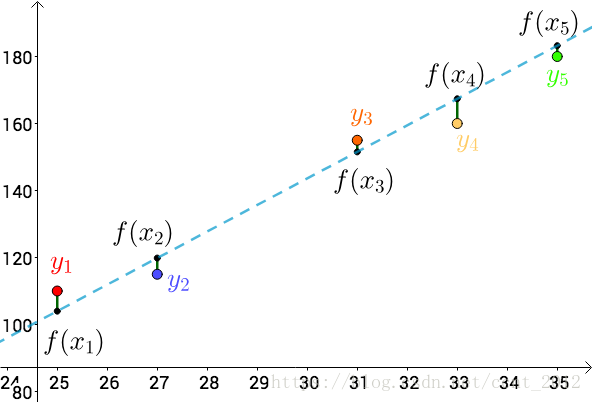
\includegraphics[width=0.9\textwidth]{./least square.png}
    \textbf{Gram-Schmidt施密特正交化(4.3最后一题)}:先将A的列正交化(即将$x_i := x_i - 1/n\sum_{i=1}^{n}x_i$),然后便可以得到对角矩阵$A^T A$,这样求$\widehat{\bm{x}}$就很方便!
    \\
    \textbf{若A的列向量线性相关}\\
    涉及到奇异值分解SVD(7.4)\\
    因为A的列向量线性相关,若把b投影到A的列空间中,即改为$A \widehat{\boldsymbol{x}}=\boldsymbol{p}$,则此时会产生多个解,即有多条直线可以选,但是不知道哪条是最佳的!
    \\
    7.4中会利用A的伪逆"pseudoinverse"来选择一个最短解$\widehat{\bm{x}}$。\\
    若A的\textbf{列线性无关},它的伪逆是$L=\left(A^{\mathrm{T}} A\right)^{-1} A^{\mathrm{T}}$
    \\
    \textbf{拟合抛物线:}\\
    同样有m个点,$(t_{1},b_{1}), \dots, (t_{m},b_{m})$,利用$C+D t+E t^{2}$来拟合这些点!\\
    $$
    \begin{aligned} C+D t_{1}+E t_{1}^{2} &=b_{1} \\ \vdots & \\ C+D t_{m}+E t_{m}^{2} &=b_{m} \end{aligned}
    \begin{array}{l}{\text { is } A \boldsymbol{x}=\boldsymbol{b} \text { with }} \\ {\text { the } m \text { by } 3 \text { matrix }}\end{array}
    A=\left[\begin{array}{ccc}{1} & {t_{1}} & {t_{1}^{2}} \\ {\vdots} & {\vdots} & {\vdots} \\ {1} & {t_{m}} & {t_{m}^{2}}\end{array}\right]
    $$
    最接近的抛物线利用$\widehat{\boldsymbol{x}}=(C, D, E)$来满足正规方程组$A^{\mathrm{T}} A \widehat{\boldsymbol{x}}=A^{\mathrm{T}} \boldsymbol{b}$。即给出了最小二乘解(具有最小均方误差MSE)。
    \\
    \textbf{解耦uncouple}:指在线性方程组中只通过一个方程就可以解出一个变量的值。\\
    \textbf{耦合couple}:指单个方程里的多个变量只能通过整个方程组来解出。
    \\
    \textbf{递归最小二乘recursive least squares}:对旧均值增加一个新数据后,不用重新计算所有值之和再除以总数,$\{b_1,\dots, b_n\}+ b_{n+1},\quad \widehat{x}_{\mathrm{new}}=\widehat{x}_{\mathrm{old}}+\frac{1}{n+1}\left(b_{n+1}-\widehat{x}_{\mathrm{old}}\right)$
    \\
    \subsection{规范(标准)正交基和施密特正交化Orthonormal Bases and Gram-Schmidt}
    当$\boldsymbol{q}_{i}^{\mathrm{T}} \boldsymbol{q}_{j}=\left\{\begin{array}{ll}{0} & {\text { when } i \neq j \quad \text { orthogonal vectors }} \\ {1} & {\text { when } i=j \quad \text { (unit vectors: }\left\|\boldsymbol{q}_{i}\right\|=1 )}\end{array}\right.$
    \quad 向量$q_{1}, \dots, q_{n}$是规范正交的。\\
    若一个矩阵的列均为规范正交向量,则记为$\bm{Q}$,有$Q^{\mathrm{T}} Q=I$。 且若$Q$是\textbf{方阵},则称其为\textbf{正交矩阵orthogonal matrix},有$Q^{\mathrm{T}}=Q^{-1}$:\textbf{转置=逆}!
    \\
    \textbf{正交矩阵的作用:}
    \begin{itemize}
        \item \textbf{旋转Rotation} \quad (二维下)$Q=\left[\begin{array}{rr}{\cos \theta} & {-\sin \theta} \\ {\sin \theta} & {\cos \theta}\end{array}\right]$将向量旋转$\theta$度; \quad $Q^{\mathrm{T}}=Q^{-1}=\left[\begin{array}{rr}{\cos \theta} & {\sin \theta} \\ {-\sin \theta} & {\cos \theta}\end{array}\right]$将向量旋转$-\theta$度。
        \item \textbf{置换Permutation} \quad 每个置换矩阵都是正交矩阵,它的逆=转置!
        \item \textbf{反射Reflection} \quad 设$\bm{u}$是任意一个单位列向量,且$Q=I-2 u u^{\mathrm{T}}$,则有$Q^{\mathrm{T}}=I-2 u u^{\mathrm{T}}=Q$,$Q^{\mathrm{T}} Q=I-4 \boldsymbol{u u}^{\mathrm{T}}+4 \boldsymbol{u} \boldsymbol{u}^{\mathrm{T}} \boldsymbol{u} \boldsymbol{u}^{\mathrm{T}}=I$,反射矩阵可以将向量$u$转为$-u$。
    \end{itemize}
    一个向量乘上正交矩阵,它的\textbf{长度,角度都不改变}:$\|Q \boldsymbol{x}\|^{2}=(Q \boldsymbol{x})^{\mathrm{T}}(Q \boldsymbol{x})=\boldsymbol{x}^{\mathrm{T}} Q^{\mathrm{T}} Q \boldsymbol{x}=\boldsymbol{x}^{\mathrm{T}} I \boldsymbol{x}=\boldsymbol{x}^{\mathrm{T}} \boldsymbol{x}=\|\boldsymbol{x}\|^{2}$,即有$\|Q \boldsymbol{x}\|=\|\boldsymbol{x}\|$;也能使点积结果不变:$(Q \boldsymbol{x})^{\mathrm{T}}(Q \boldsymbol{y})=\boldsymbol{x}^{\mathrm{T}} Q^{\mathrm{T}} Q \boldsymbol{y}=\boldsymbol{x}^{\mathrm{T}} \boldsymbol{y}$
    \subsubsection{用规范正交基做投影,Q代替A}
    对于投影到子空间,通常利用$A^T A$,$A^T A$中的条目为$\boldsymbol{a}_{i}^{\mathrm{T}} \boldsymbol{a}_{j}$,即A的基的点积。\\
    \textbf{现假设A的基是规范正交的},则$A^T A$简化为$Q^T Q=I$(解耦了),且:
    \begin{itemize}
        \item $Q^T Q\widehat{\boldsymbol{x}}=Q^{\mathrm{T}} \boldsymbol{b} \rightarrow \widehat{\boldsymbol{x}}=Q^{\mathrm{T}} \boldsymbol{b}$
        \item $\bm{p}=Q \widehat{\bm{x}} = Q Q^{\mathrm{T}} \bm{b}$
        \item $P=Q(Q^T Q)^{-1}Q^{\mathrm{T}} \rightarrow P=Q Q^T$
    \end{itemize}
    $\boldsymbol{p}=Q Q^{\mathrm{T}} \bm{b}=\left[\begin{array}{lll}{|} & {} & { |} \\ {\bm{q}_{1}} & {\cdots} & {\bm{q}_{n}} \\ { |} & {} & { |}\end{array}\right]\left[\begin{array}{c}{\bm{q}_{1}^{\mathrm{T}} \bm{b}} \\ {\vdots} \\ {\bm{q}_{n}^{\mathrm{T}} \bm{b}}\end{array}\right]=\boldsymbol{q}_{1}\left(\boldsymbol{q}_{1}^{\mathrm{T}} \boldsymbol{b}\right)+\cdots+\boldsymbol{q}_{n}\left(\boldsymbol{q}_{n}^{\mathrm{T}} \boldsymbol{b}\right)$
    \\
    当Q为方阵时,列空间便为整个空间,$Q^{\mathrm{T}}=Q^{-1}$,$\boldsymbol{x}=Q^{-1} \boldsymbol{b}$,最小二乘解是精确的,$\bm{b}$在整个空间上的投影是它自己,$P=Q Q^{\mathrm{T}}=I$。
    \\
    $\boldsymbol{p}=\boldsymbol{b}=Q Q^{\mathrm{T}} \bm{b}=\bm{q}_{1}\left(\bm{q}_{1}^{\mathrm{T}} \bm{b}\right)+\bm{q}_{2}\left(\bm{q}_{2}^{\mathrm{T}} \bm{b}\right)+\cdots+\bm{q}_{n}\left(\bm{q}_{n}^{\mathrm{T}} \bm{b}\right)$,这说明了每个$\bm{b}$是沿着Q的基方向的每个$\bm{b}$的分量之和!$\widehat{\bm{x}}_i = \bm{q}^T_{i} \bm{b}, \quad \bm{q}_i \widehat{\bm{x}}_i$\textbf{是向量b在第i个基上的投影!故每个基上的投影加起来便是原向量b!(用于QR分解的理解!)}
    \\
    $Q Q^{\mathrm{T}}=I$是傅里叶变换基础,这些变换将向量或者函数分解成垂直片断,再通过上式利用逆变换将这些片段放到一起组成向量或者函数f。

    \subsubsection{施密特正交化}
    思想:新向量减去它在已有的正交向量上的投影向量,即求误差$e$,这就是新的正交向量!最后对每个正交向量除以自己的长度,进行归一化!

    \subsubsection{$A_{m\times n}=Q_{m\times m}R_{m\times n}$分解}
    具体表述以及推导过程参考\url{https://blog.csdn.net/u010945683/article/details/45972819}(\textbf{QR分解解析}),
    里面将从施密特正交化求正交基的方法中将转换前和转换后的向量用线性组合表示出来,然后再写成矩阵乘法形式,清晰易懂。

    将上述的A与Q(规范正交矩阵)用R(上三角矩阵)联系起来,\textbf{A--->施密特正交化--->Q},每一步$\boldsymbol{a}_{1}, \dots, \boldsymbol{a}_{k}$都是$q_{1}, \ldots, q_{k}$的线性组合,后面的$\bm{q}_{k+1}...$均不涉及。正交化过程中用到的转换矩阵便是$T,R=T^{-1}$。

    $A=Q R=$
    $\left[\begin{array}{lll}{\bm{a}} & {\bm{b}} & {\bm{c}}\end{array}\right]=\left[\begin{array}{lll}{\bm{q}_{1}} & {\bm{q}_{2}} & {\bm{q}_{3}}\end{array}\right]\left[\begin{array}{ccc}{\bm{q}_{1}^{T} \bm{a}} & {\bm{q}_{1}^{T} \bm{b}} & {\bm{q}_{1}^{T} \bm{c}} \\ {} & {\bm{q}_{2}^{T} \bm{b}} & {\bm{q}_{2}^{T} \bm{c}} \\ {} & {} & {\bm{q}_{3}^{T} \bm{c}}\end{array}\right]$

    简而言之,$A=Q R$就是Gram-Schmidt正交化的产物,左乘一个$Q^T$得:$\boldsymbol{R}=\boldsymbol{Q}^{\mathrm{T}} \boldsymbol{A}$,其中$R$为上三角矩阵!(因为$Q^T Q = I$)

    \subsubsection{Problem set}
    4. (a) Any $Q_{m\times n}$ with $n<m$ has $Q Q^{\mathrm{T}} \neq I$,如$Q=\left[\begin{array}{ll}{1} & {0} \\ {0} & {1} \\ {0} & {0}\end{array}\right], Q Q^{\mathrm{T}}=\left[\begin{array}{ccc}{1} & {0} & {0} \\ {0} & {1} & {0} \\ {0} & {0} & {0}\end{array}\right] \neq I$
    \\
    若A能QR分解,则$A^{\mathrm{T}} A=R^{\mathrm{T}} R$下三角乘上三角。